
\section{Influence of Model Parameters}\label{sec:expparam}
This section presents experimental results concerning the influence of several model parameters. The model presented in this work has a variety of different parameters that can have an influence on its performance. These parameters concern:
\begin{description}
\item[Training data:] \hfill 
\begin{itemize}
\item The amount of training data
\item Synthetic vs. real vs. mixed data
\item Orthographic vs. perspective CAD rendering
\item Backgrounds of rendered CAD examples (negative examples vs. mean pixels)
\item Angle $\alpha$ for which an example's viewpoint is fixed during training
\end{itemize}
\end{description}

\begin{description}
\item[Model:] \hfill 
\begin{itemize}
\item Number of views/mixture components
\item Number of 3D parts
\item Number of visible parts per viewpoint
\item Rootfilter dimension/area
\item Number of elevations the model is trained on
\end{itemize}
\end{description}

\begin{description}
\item[Learning:] \hfill 
\begin{itemize}
\item L-SVM parameters C and J (cost weighting factor for positive examples)
\item Influence of incorrect viewpoint penalty
\end{itemize}
\end{description}

\begin{description}
\item[Features:] \hfill 
\begin{itemize}
\item HOG vs. CNN
\item Truncation feature
\item Standardisation of CNN features
\item Extra octave for feature pyramid
\end{itemize}
\end{description}

To test the influence of some of these parameters and maximise performance of the model, experiments were conducted on the VOC 2012 validation data. For most of the experiments, all but one parameter were kept fixed and a model was trained with different values for the given parameter. After evaluating the performance of the model on the validation set, the best performing parameter value was chosen and fixed during experiments with other parameters.  Both average precision as measured by the VOC criteria (a minimum of 0.5 bounding box overlap) and viewpoint accuracy (0.5 overlap and correct viewpoint) proposed by \cite{xiang_wacv14} were used as performance measures. Tables \ref{tab:modelParam}-\ref{tab:otherParam} show the results for some parameters as relative performance loss or gain for different values. 

%
\begin{table}[]
	\parbox{.45\linewidth}{
		\centering
		\begin{tabular}{|c|c|c|}
		\hline
		 Root Area & AP & VA \\
		\hline\hline
		 57-67 & 0 & 0  \\
		\hline 
		 62-72 & +1.1 & +1.4 \\
		\hline
		 67-77 & +0.4 & +0.2 \\
		\hline
		\end{tabular}
		\subcaption{Relative AP and VA for different root area constraints (min-max)}
		\label{tab:rootarea}
	}		
	%
	\parbox{.45\linewidth}{
		\centering
		\begin{tabular}{|c|c|c|}
		\hline
		 \#Components & AP & VA\\
		\hline\hline
		 4 & 0 & 0\\
		\hline 
		 8  & +1.2 & +0.6 \\
		 \hline 
		 16 & -0.7 & -6.2\\
		 \hline
		\end{tabular}
		\subcaption{Relative AP and VA for different numbers of mixture components}
		\label{tab:numComp}
	}		
	%
	\parbox{\linewidth}{
		\centering
		\begin{tabular}{|c|c|c|c|}
		\hline
		 \#3D parts & Max parts per view & AP & VA\\
		\hline\hline
		 12 & 8 & 0  & 0\\
		\hline 
		 16 & 10 & +0.4 & -0.3\\
		 \hline 
		 20 & 12 & +1.2 & +0.8\\
		 \hline
		\end{tabular}
		\subcaption{Relative AP and VA for different numbers of 3D-parts and parts per view (PpV)}
		\label{tab:parts}
	}	
	%
	\parbox{.5\linewidth}{
		\centering
		\begin{tabular}{|c|c|c|c|}
		\hline
		 \#elevations & AP & VA\\
		\hline\hline
		 1 & 0  & 0\\
		\hline 
		 2 & -0.9 & -0.6\\
		 \hline 
		\end{tabular}
		\subcaption{Relative AP and VA for different numbers of elevations}
		\label{tab:elev}
	}
	%
	\parbox{.5\linewidth}{
		\centering
		\begin{tabular}{|c|c|c|c|}
		\hline
		 Extra pyramid octave & AP & VA\\
		\hline\hline
		 without & 0  & 0\\
		\hline 
		 with & +5.2 & +3.1\\
		 \hline 
		\end{tabular}
		\subcaption{Relative AP and VA for models with or without an extra pyramid octave}
		\label{tab:extraoctave}
	}
	\caption{Tables showing the influence of several model parameters on average precision (AP) and average viewpoint accuracy (VA).}
	\label{tab:modelParam}
\end{table}
%
Table \ref{tab:rootarea} illustrates the influence of the constraints on the model's root filter areas in feature dimensions. We can observe that the performance decreases for areas of sizes between 57 and 67 or 67 and 77 compared to  root filter areas  of sizes between  62 and 72. Smaller root areas lead to filters that do not capture enough detail and therefore might miss some meaningful details of the object's appearance. As root filter areas have a direct influence on the size of the smallest perceivable object instances, bigger root filters lead to fewer detections of small objects. 

The influence of the number of mixture-components/views can be observed in table \ref{tab:numComp}. Note that viewpoint accuracy (VA) decreases significantly when increasing number of views from 8 to 16. This is expected as more views lead to a finer binning of viewpoints and neighbouring viewpoints therefore get more difficult to discriminate. We can also observe that detection performance increases when going from 4 views to  8. This can be explained by a more complex model and an increased variety of aspect ratios covered by the root filters. The slight decrease in performance when going from 8 views to 16 could be explained by the fact that more model components result in a reduction of training examples for each component. 

The influence of different amounts of parts can be seen in table \ref{tab:parts}. We see that increasing the number of parts generally increases the performance of the model. Note that by construction (section \ref{sec:partInit}) more 3D parts lead to smaller 2D part-templates. Also, the model's complexity doesn't increase by much  as part filters are only added until no more root filter area can be covered by new parts. Therefore the model effectively just grows from the additional deformation parameters. 

Surprisingly, training models on more than one elevation didn't lead to better performance (table \ref{tab:elev}). A possible explanation for this observation could be found in the distribution of object viewpoints in the data sets (see figure \ref{fig:hist}). As there are not many examples having an increased elevation there are not a lot of training examples for the new components and the training data of the more important (ground-level) views is reduced.

One of the most significant boosts in performance was observed when training the model with an extra octave added to the feature  pyramid (table \ref{tab:extraoctave}). The highest resolution feature maps computed on an extra octave pyramid are computed at four times the resolution of the original image. This modification leads to more training examples, as some examples were just too small to be used with the normal pyramid, and also allows the model to detect smaller object instances at test time. It should be noted however that this performance gain come at the cost of increased detection and training time. 

\begin{table}[]
	\parbox{.45\linewidth}{
		\centering
		\begin{tabular}{|c|c|c|}
		\hline
		Training data & AP & VA\\
		\hline\hline
		 Real only & 0 & 0\\
		\hline 
		 Real+CAD persp. & -1 & -0.6 \\
		 \hline 
		 Real+CAD ortho. & -1.9 & -2\\
		 \hline
		\end{tabular}
		\subcaption{Relative AP and VA for different training data}
		\label{tab:data}
	}		
	%
	\parbox{.45\linewidth}{
		\centering
		\begin{tabular}{|c|c|c|}
		\hline
		Fixation angle $\alpha$ & AP & VA\\
		\hline\hline
		 20 & 0 & 0\\
		\hline 
		 45  & -1 & +0.2 \\
		 \hline 
		 5 & -0.5 & -0.4 \\
		 \hline
		\end{tabular}
		\subcaption{Relative AP and VA for different viewpoint fixation angles.}
		\label{tab:alpha}
	}	
	\parbox{\linewidth}{
		\centering
		\begin{tabular}{|c|c|c|}
		\hline
		CAD background& AP & VA\\
		\hline\hline
		 Negative training images & 0 & 0\\
		\hline 
		 Mean pixels of CNN features & +0.8 & +2.3 \\
		 \hline 
		\end{tabular}
		\subcaption{Relative AP and VA for different backgrounds of the CAD training examples}
		\label{tab:background}
	}
	\caption{Tables showing the influence of training data parameters.}
	\label{tab:dataParam}
\end{table}

In table \ref{tab:data} we can observe the influence of different training data configurations. Note that training a model on only real training data implies that no 3D-constraints can be enforced on the model and parts are learnt fully independent across views. This can be one explanation why there is an improvement in performance compared to training on a combination of synthetic and real images, as parts can be learnt optimally for each separate view. Also, the importance of using perspective projections for rendering becomes apparent. While orthographic projections are a reasonable approximation for far away objects, real images of cars often are taken from a rather close distance. As table \ref{tab:background} shows, uniform backgrounds showed to work better than backgrounds of negative training images.  

The influence of the angle $\alpha$ which defines the range of viewpoints that are going to be assigned to a fixed mixture component during training is shown in table \ref{tab:alpha}. The choices for $\alpha$ here are listed for a four-component-model and of course $\alpha=min(\alpha,360/(2*\#Comp))$ holds. As expected a value of $\alpha=45$, which means in this case that all examples are fixed to their correct viewpoint, increases viewpoint accuracy but decreases detection performance significantly. More surprising is that an angle of 5 decreases performance in both tasks compared to an angle of 20. 

\begin{table}[]
	\parbox{.45\linewidth}{
		\centering
		\begin{tabular}{|c|c|c|}
		\hline
		Penalty term $l$ & AP & VA\\
		\hline\hline
		 without & 0 & 0\\
		\hline 
		 with & +0.5 & +2.8 \\
		 \hline 
		\end{tabular}
		\subcaption{Relative AP and VA influence of penalty term.}
		\label{tab:penalty}
	}	
	%	
	\parbox{.45\linewidth}{
		\centering
		\begin{tabular}{|c|c|c|}
		\hline
		Truncation feature & AP & VA\\
		\hline\hline
		 without & 0 & 0\\
		\hline 
		 with & +7.9 & +7.5 \\
		 \hline 
		\end{tabular}
		\subcaption{Relative AP and VA influence of penalty term.}
		\label{tab:truncfeat}
	}		
	\caption{Tables showing the influence of penalty term and truncation feature.}
	\label{tab:otherParam}
\end{table}

As we can see from table \ref{tab:penalty} the penalty term $l$, introduced to softly enforce the correct viewpoints (equation \ref{eq:penalty}), does not only deliver a better viewpoint-estimation performance but also slightly raises detection performance. Again, we observe that correct viewpoint assignments favour the detection performance. Table \ref{tab:truncfeat} shows the significant performance boost obtained by the truncation feature and the related adjustments described in section \ref{sec:trunc}.

\begin{table}[]
\resizebox{0.7\linewidth}{!}{\begin{minipage}{\textwidth}
	\begin{center}
		\begin{tabular}{|c|c|c|c|c|c|c|}
		\hline
		 3D-DPM & 3D-DPM+ & DPMver3 \cite{5255236} & DPMver4 \cite{voc-release4} & DPM-VOC \cite{6248075} & DPM 3D-Const. \cite{6248075} & 3D2PM \cite{Pepik:2012aa}\\
		\hline\hline
		53.9 & 63.4 & 50.2 & 57.9 & 66 & 63.1 & 61.2\\
		\hline
		\end{tabular}
	\end{center}
\end{minipage} }
\caption{Average Precision (AP) on cars of the VOC 2007 \cite{pascal-voc-2007} test set. Results for the model in this project are given in the first two columns and results of other models are provided for comparison.}\label{tab:voc2007}
\end{table}

%\begin{table}[]
%\resizebox{\linewidth}{!}{\begin{minipage}{\textwidth}
%	\begin{center}
%		\begin{tabular}{|c|c|c|c|}
%		\hline
%		3D-DPM & DPM & DPM 3D-Const. & 3D2PM\\
%		\hline\hline
%		63.4 & 57.9 & 63.1 & 61.2\\
%		\hline
%		\end{tabular}
%	\end{center}
%\end{minipage} }
%\caption{Average Precision (AP) on cars of the VOC 2007 \cite{pascal-voc-2007} test set. Results for the model in this project are given in the first two columns and results of other models are provided for comparison.}\label{tab:voc2007}
%\end{table}

\section{Bounding Box Localisation}\label{sec:boxloc}
To test the model's detection performance the model was evaluated on the well known and challenging Pascal VOC 2007 \cite{pascal-voc-2007} dataset, the VOC 2012 \cite{pascal-voc-2012} 'val' set, and the 3D object dataset \cite{4408987}.   The performance measure used is the standard VOC measure of a minimum ground truth bounding box overlap of 50\%.

Table \ref{tab:voc2007} reports the results on VOC 2007 of the model implemented in this project (3D-DPM and 3D-DPM+) and also lists results for different versions of the DPM and similar models. 3D-DPM is an eight-view-model  which was trained on perspective CAD examples and real training images from VOC 2007 'trainval'. 3D-DPM+ was trained on additional training data from VOC2012 'train', the first five car models of 3D object dataset and uses an extra octave pyramid. 

We see that the 3D-DPM outperforms DPMver3 on which it is built upon and doesn't quite perform as good as DPMver4. The performance improvements with respect to DPMver3 can largely be attributed to the addition of the truncation feature, as well as the higher number of components. A possible explanation for the performance difference to DPMver4 could lie in the fact that VOC 2007 examples come without viewpoint annotations and therefore the model is initialised on CAD examples only (which might lead to sub-optimal filter dimensions and initialisations). Using additional examples from VOC 2012 in fact showed to increase the performance to around the same value as DPMver4 achieves. Another explanation can be found in the 3D constraints, which have already showed to have a negative impact on detection performance.

Compared to the other 3D DPM implementations DPM 3D-Constraints \cite{6248075} and 3D2PM \cite{Pepik:2012aa}, 3D-DPM performs worse. On the other hand, the performance boost of 3D-DPM+ obtained by the use of an extra pyramid octave lifts its performance above the ones reported for the other two 3D models \cite{Pepik:2012aa} \cite{6248075}. This suggests that these models most probably also made use of an extra octave pyramid, an implementation detail not mentioned in their publications. As \cite{6248075} report an average precision of 63.3 on VOC 2007 cars without the SSVM formulation and without the addition of synthetic training data, no other design choice seems to justify the performance difference to 3D-DPM or DPMver4. 

\begin{table}[]
\resizebox{1\linewidth}{!}{\begin{minipage}{\textwidth}
	\begin{center}
		\begin{tabular}{|c|c|c|c|c|}
		\hline
		\#views & 3D-DPM & 3D-DPM+ & VDPM \cite{xiang_wacv14} & DPM-VOC+VP \cite{6248075}\\
		\hline\hline
		4 &  38.2/30.2 & 47.4/37.3 & 37.2/20.2 & 45.6/36.9\\
		\hline
		8 &  39.4/30.8 & 49.4/35.5 & 37.3/23.5 & 47.6/36.6\\
		\hline
		16 & 37.5/24.0 & 47.5/29.5 & 36.6/18.1 & 46.0/29.6\\
		\hline
		\end{tabular}
	\end{center}
\end{minipage} }
\caption{Average precision and average viewpoint accuracy (AP/VA) on cars of the VOC 2012 'val' set with annotations by \cite{xiang_wacv14}.}\label{tab:voc2012}
\end{table}

Table \ref{tab:voc2012} lists the AP of 3D-DPM and 3D-DPM+ on the VOC2012 'val' dataset. It also shows results for DPM-VOC+VP \cite{Pepik:2012aa} and VDPM which is a modification of DPMver4 in which root filters are initialised on training sets that are obtained by binning the annotated VOC2012 test data of \cite{xiang_wacv14} into $k$ viewpoint bins. After the initialisation on the correct viewpoints, training is identical to the standard DPM training of DPMver4. Here, we observe that 3D-DPM achieves consistently higher average precision compared to VDPM (DPMver4) and considerably worse than DPM-VOC+VP. On the other hand, 3D-DPM+ achieves the highest average precision of all the listed models. Some of the performance gain compared to DPM-VOC+VP might be due to the higher amount of training data.

\begin{table}[]
\resizebox{0.9\linewidth}{!}{\begin{minipage}{\textwidth}
	\begin{center}
		\begin{tabular}{|c|c|c|c|c|}
		\hline
		3D-DPM & 3D-DPM+ & DPM 3D-Const. \cite{6248075} & 3D2PM \cite{Pepik:2012aa} & DPM-VOC+VP \cite{6248075}\\
		\hline\hline
		99.1/96.7 & 98.2/93.3 & 99.7/96.3 & 99.6/95.8 & 99.9/97.9\\
		\hline
		\end{tabular}
	\end{center}
\end{minipage} }
\caption{Average precision and viewpoint estimation in MPPE on cars of the 3D Object classes dataset \cite{4408987}.}	\label{tab:3DDataset}
\end{table}

Finally, the results on the 3D object classes dataset \cite{4408987} are shown in table \ref{tab:3DDataset}. This is a rather easy dataset as all the cars are in full sight and the viewpoints exactly match the viewpoints an eight-view-model is trained on. For comparison the results for other models are listed as well. Note however, that for these models it is unclear which of the examples in the dataset were used for testing. While they state that a subset of the examples was used for training, the exact assembly and size of the subset is unknown, making the comparison difficult. 3D-DPM is trained on CAD renderings, examples from VOC2012 and the first five (of ten) car models of the 3D object dataset. The last five car models were used for testing. It is interesting to notice that 3D-DPM+ performs slightly worse than 3D-DPM on this occasion. As the dataset is also relatively small (only 480 car examples in total), these performance differences should be taken with a grain of salt. Overall, the performance is comparable to the other models.

%\begin{figure}
%\begin{center}
%        \begin{subfigure}[b]{0.49\textwidth}
%                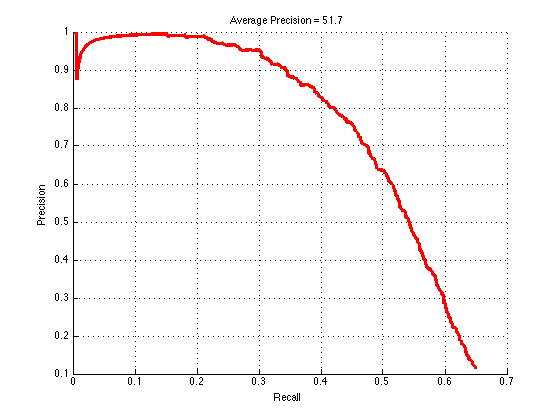
\includegraphics[width=\textwidth]{voc20074comp}
%               	\caption{VOC 2007 4 views}
%        \end{subfigure}
%        \begin{subfigure}[b]{0.49\textwidth}
%                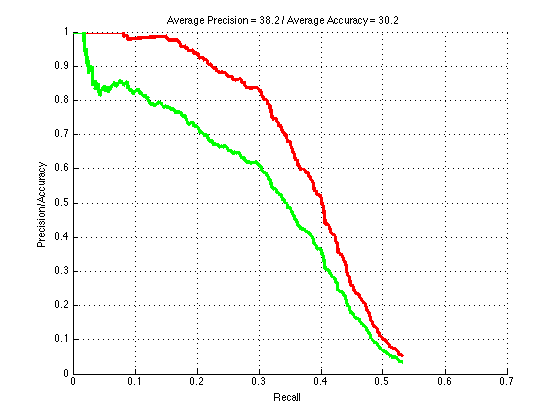
\includegraphics[width=\textwidth]{voc20124comp}
%                \caption{VOC2012 4 views}
%        \end{subfigure}
%        \begin{subfigure}[b]{0.49\textwidth}
%                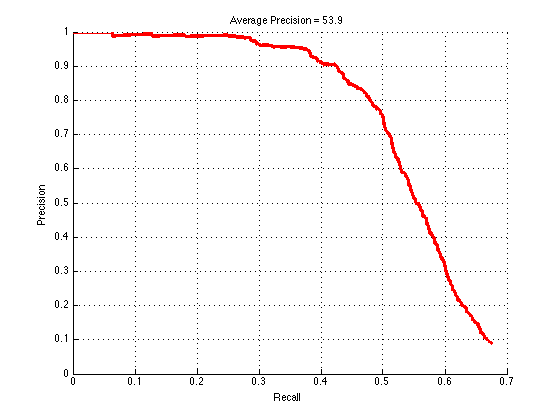
\includegraphics[width=\textwidth]{voc20078comp}
%               	\caption{VOC 2007 8 views}
%        \end{subfigure}
%        \begin{subfigure}[b]{0.49\textwidth}
%                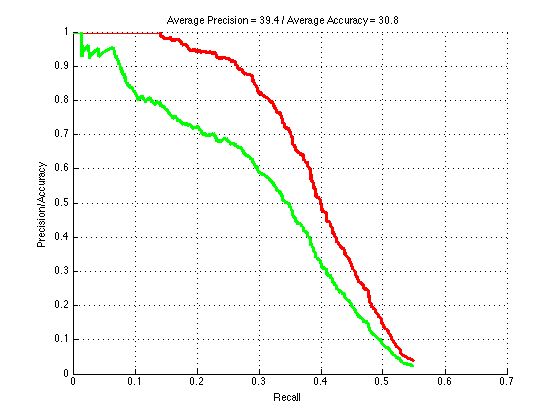
\includegraphics[width=\textwidth]{voc20128comp}
%                \caption{VOC2012 8 views}
%        \end{subfigure}
%        \begin{subfigure}[b]{0.49\textwidth}
%                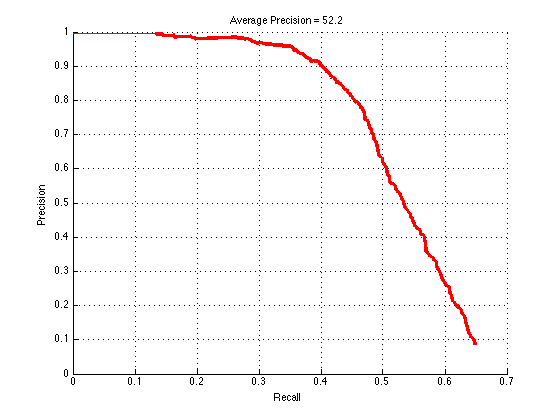
\includegraphics[width=\textwidth]{voc200716comp}
%               	\caption{VOC 2007 16 views}
%        \end{subfigure}
%        \begin{subfigure}[b]{0.49\textwidth}
%                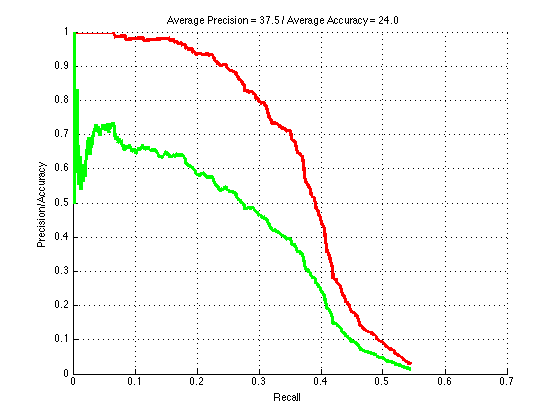
\includegraphics[width=\textwidth]{voc201216comp}
%                \caption{VOC2012 16 views}
%        \end{subfigure}        
%\caption{Precision-Recall curves of 3D-DPM on VOC 2007 'test' (left) and Precision/Accuracy-Recall curve on VOC 2012 'val' (right). }
%\label{fig:3ddpm}
%\end{center}
%\end{figure}
%
%\begin{figure}
%\begin{center}
%        \begin{subfigure}[b]{0.49\textwidth}
%                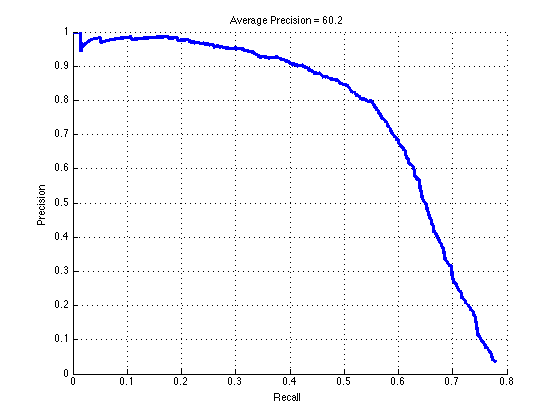
\includegraphics[width=\textwidth]{voc2007best4}
%               	\caption{VOC 2007 4 views}
%        \end{subfigure}
%        \begin{subfigure}[b]{0.49\textwidth}
%                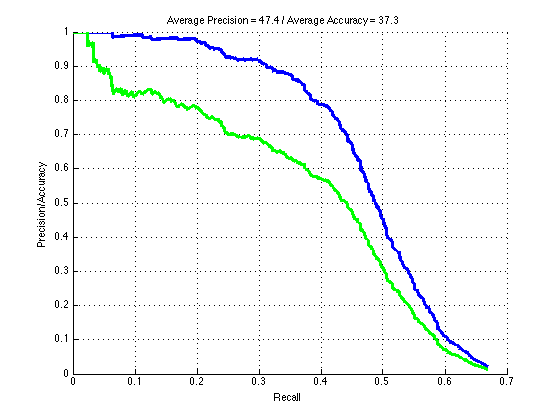
\includegraphics[width=\textwidth]{voc2012best4}
%                \caption{VOC2012 4 views}
%        \end{subfigure}
%        \begin{subfigure}[b]{0.49\textwidth}
%                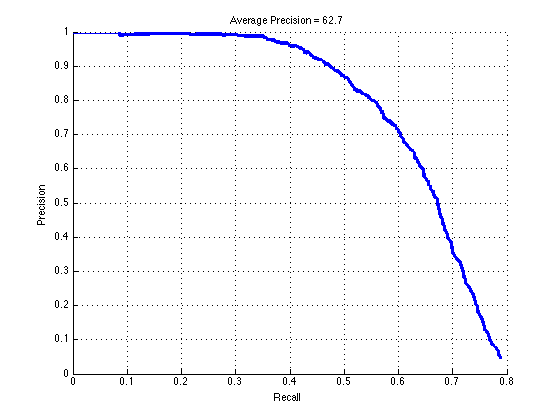
\includegraphics[width=\textwidth]{voc2007best8}
%               	\caption{VOC 2007 8 views}
%        \end{subfigure}
%        \begin{subfigure}[b]{0.49\textwidth}
%                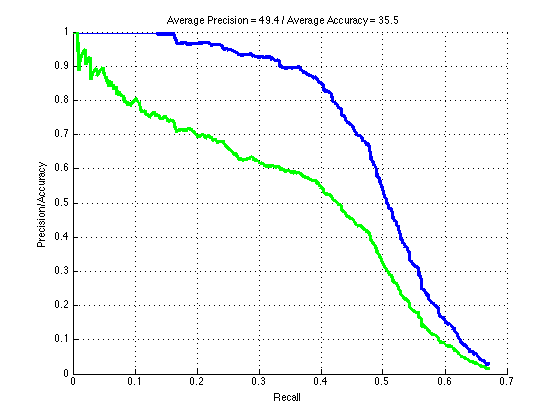
\includegraphics[width=\textwidth]{voc2012best8}
%                \caption{VOC2012 8 views}
%        \end{subfigure}
%        \begin{subfigure}[b]{0.49\textwidth}
%                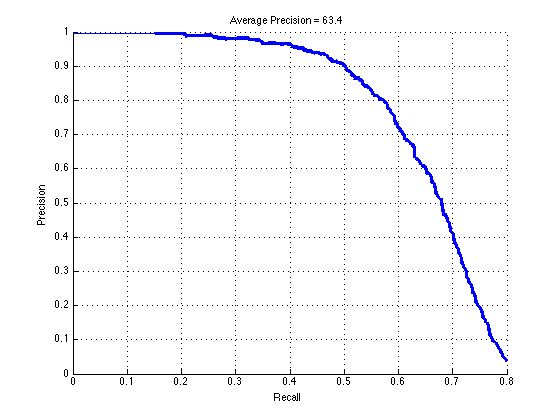
\includegraphics[width=\textwidth]{voc2007best16}
%               	\caption{VOC 2007 16 views}
%        \end{subfigure}
%        \begin{subfigure}[b]{0.49\textwidth}
%                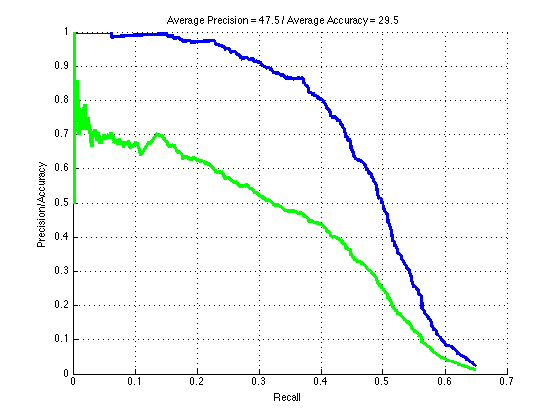
\includegraphics[width=\textwidth]{voc2012best16}
%                \caption{VOC2012 16 views}
%        \end{subfigure}        
%\caption{Precision-Recall curves of  3D-DPM+ on VOC 2007 'test' (left) and Precision/Accuracy-Recall curves on VOC 2012 'val' (right). }
%\label{fig:3ddpm+}
%\end{center}
%\end{figure}

% new PR figures

\begin{figure}
\begin{center}
	\begin{subfigure}[b]{0.49\textwidth}
       		\includegraphics[width=\textwidth]{3DdatasetPR}       
                \caption{3D-DPM}
        \end{subfigure}
        \begin{subfigure}[b]{0.49\textwidth}
       		\includegraphics[width=\textwidth]{3DdatasetVA}       
       		\caption{3D-DPM+}
        \end{subfigure}
%        \begin{subfigure}[b]{0.49\textwidth}
%       		\includegraphics[width=\textwidth]{3DdatasetPRbest}       
%                \caption{3D-DPM+}
%        \end{subfigure}
\caption{Precision/Recall (left) and Viewpoint-Accuracy/Recall (right) curves on cars of the 3D object dataset \cite{4408987} of models described in this project. All the models were trained using all the training data (CAD, VOC2007, VOC2012, 3D Dataset). 3D-DPM+ uses an extra octave pyramid and 3D-DPM PN uses positive training data with wrong viewpoint labels as negative training examples.}
\label{fig:PR3DDataset}
\end{center}
\end{figure}

\begin{figure}
\begin{center}
        \begin{subfigure}[b]{0.49\textwidth}
                \includegraphics[width=\textwidth]{voc2007PR4}
               	\caption{VOC 2007 4 views}
        \end{subfigure}
        \begin{subfigure}[b]{0.49\textwidth}
                \includegraphics[width=\textwidth]{voc2012PR4}
                \caption{VOC2012 4 views}
        \end{subfigure}
        \begin{subfigure}[b]{0.49\textwidth}
                \includegraphics[width=\textwidth]{voc2007PR8}
               	\caption{VOC 2007 8 views}
        \end{subfigure}
        \begin{subfigure}[b]{0.49\textwidth}
                \includegraphics[width=\textwidth]{voc2012PR8}
                \caption{VOC2012 8 views}
        \end{subfigure}
        \begin{subfigure}[b]{0.49\textwidth}
                \includegraphics[width=\textwidth]{voc2007PR16}
               	\caption{VOC 2007 16 views}
        \end{subfigure}
        \begin{subfigure}[b]{0.49\textwidth}
                \includegraphics[width=\textwidth]{voc2012PR16}
                \caption{VOC2012 16 views}
        \end{subfigure}        
\caption{Precision-Recall curves on VOC 2007 'test' (left) and on VOC 2012 'val' (right).  All the models were trained using all the training data.  }
\label{fig:PRVOC}
\end{center}
\end{figure}

\begin{figure}
\begin{center}
        \begin{subfigure}[b]{0.49\textwidth}
                \includegraphics[width=\textwidth]{voc2012VA4}
               	\caption{3D-DPM CNN 4 views}
        \end{subfigure}
        \begin{subfigure}[b]{0.49\textwidth}
                \includegraphics[width=\textwidth]{voc2012VA8}
               	\caption{3D-DPM CNN 8 views}
        \end{subfigure}
        \begin{subfigure}[b]{0.49\textwidth}
                \includegraphics[width=\textwidth]{voc2012VA16}
               	\caption{3D-DPM CNN 16 views}
        \end{subfigure}        
    \caption{Viewpoint-Accuracy-Recall curves on VOC 2012 'val' of models described in this project. Only examples with bounding-box overlap of at least 0.5 and correct viewpoint label are considered correctly classified. All the models were trained using all the training data (CAD, VOC2007, VOC2012, 3D Dataset). 3D-DPM+ uses an extra octave pyramid and 3D-DPM PN uses positive training data with wrong viewpoint labels as negative training examples.}
\label{fig:AVVOC2012}
\end{center}
\end{figure}

\section{Viewpoint Estimation}

To test the model's performance on pose-estimation, experiments on the 3D object dataset as well as the VOC 2012 'val' set with the viewpoint annotations from \cite{xiang_wacv14} were conducted. The performance measures used were viewpoint accuracy (VA) and mean precision in pose-estimation (MPPE). Viewpoint accuracy only counts detections with a minimum bounding box overlap of 50\% and a correct viewpoint assignment as valid detections, therefore measuring the combination of both, object localisation and viewpoint estimation. MPPE is defined as the average along the diagonal of the viewpoint confusion matrix, therefore ignoring correct bounding box localisation altogether. 

Table \ref{tab:voc2012} lists results on the 3D object category dataset in MPPE. 3D-DPM was trained using CAD renderings, examples from VOC 2012 and the first five cars of the 3D object category dataset. 3D-DPM+ again used all the training examples and makes use of an extra octave pyramid. Results for other 3D Deformable Parts Models  \cite{6248075} \cite{Pepik:2012aa} and DPM-VOC+VP \cite{6248075} are listed for comparison. Note however that the test sets might differ (see section  \ref{sec:boxloc}). The MPPE achieved by 3D-DPM is slightly higher than the results reported by the other 3D models and not quite as good as the results obtained by DPM-VOC+VP. Interestingly however, 3D-DPM+ performs worse than the other models on this dataset. 


The viewpoint accuracy results on VOC 2012 are listed in table \ref{tab:voc2012}. For comparison the results reported for DPM-VOC+VP and VDPM (DPMver4 initialised on correct viewpoints) are shown as well. By comparing the results of 3D-DPM to VDPM (which both use the same pyramid), we can observe the drastic improvement in viewpoint accuracy obtained by the continuous enforcement of correct viewpoints during training through component-fixation and the penalty term. The results for 3D-DPM+ show a significant improvement in viewpoint accuracy compared to 3D-DPM. This improvement is mainly due to the better detection performance and does not imply that 3D-DPM+ obtains better viewpoint estimation given a correct detection. The results achieved by  3D-DPM+ are nearly identical to the results obtained by DPM-VOC+VP \cite{6248075}.

\section{CNN vs. HOG Features}\label{sec:cnnexp}	

This section will present the influence of several design choices on the performance of a CNN based model, report results obtained with such models and compare the performance of a CNN based model to HOG based models. 

\begin{table}[]
	\begin{center}
		\begin{tabular}{|c|c|c|}
		\hline
		Feature standardisation & AP & VA\\
		\hline\hline
		 without & 0 & 0\\
		\hline 
		 with & +22 & +21.5 \\
		 \hline 
		\end{tabular}
	\end{center}
	\caption{Relative AP and VA with or without feature standardisation}
	\label{tab:featStand}
\end{table}

\begin{table}[]
	\begin{center}
		\begin{tabular}{|c|c|c|}
		\hline
		Lower bounds on deformations & AP & VA\\
		\hline\hline
		 $(0.01, 0, 0.01, 0)$ & 0 & 0\\
		\hline 
		 $(0.2, 0, 0.2, 0)$ & +7.6 & +8.4 \\
		 \hline 
		\end{tabular}
	\end{center}
	\caption{Relative AP and VA for different lower-bounds}
	\label{tab:lowerbound}
\end{table}

Table \ref{tab:featStand} lists the relative performance gain on the VOC2012 'val' set achieved through feature standardisation and table \ref{tab:lowerbound} shows the influence of the increased deformation lower-bounds. The importance of these modifications is obvious from the experiments. As mentioned in section \ref{sec:cnnFeat}, feature standardisation mainly improves the SVM training while the increased lower-bounds are important to prevent parts from moving too far away from their anchor positions. 

\begin{table}[]
	\begin{center}
		\begin{tabular}{|c|c|c|}
		\hline
		\#views & 3D-DPM CNN & 3D-DPM HOG\\
		\hline\hline
		4 &  55.3  & 54.3\\
		\hline
		8 & 53.1 &  54.7\\
		\hline
		16 & 51.8 &  57.1 \\
		\hline
		\end{tabular}
	\end{center}
\caption{Comparing the detection performance of a CNN based model to a HOG based model using average precision on cars of the VOC 2007 'test' set.}\label{tab:cnn2007}
\end{table}

%\begin{figure}
%\begin{center}
%        \begin{subfigure}[b]{0.49\textwidth}
%                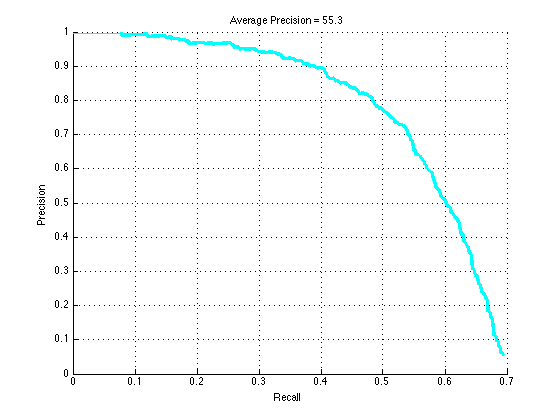
\includegraphics[width=\textwidth]{voc2007PRcnn4}
%               	\caption{3D-DPM CNN 4 views}
%        \end{subfigure}
%        \begin{subfigure}[b]{0.49\textwidth}
%                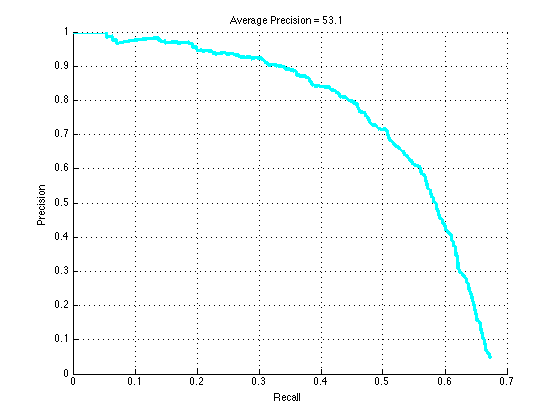
\includegraphics[width=\textwidth]{voc2007PRcnn8}
%               	\caption{3D-DPM CNN 8 views}
%        \end{subfigure}
%        \begin{subfigure}[b]{0.49\textwidth}
%                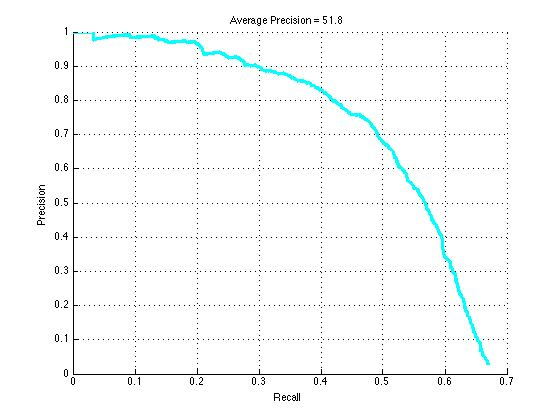
\includegraphics[width=\textwidth]{voc2007PRcnn16}
%               	\caption{3D-DPM CNN 16 views}
%        \end{subfigure}        
%    \caption{Precision/Accuracy-Recall curves on VOC 2007 'test' of 3D-DPM CNN (left) and 3D-DPM CNN-PN (right). }
%\label{fig:voc2007cnn}
%\end{center}
%\end{figure}

Results for a CNN-based model on VOC 2007 'test' are listed in table \ref{tab:cnn2007}. For comparison, the results of a HOG-based 3D-DPM are also shown. Both these models were trained using all the training data. 3D-DPM CNN is trained using badly localised positives as negatives in addition to the normal negative training examples. Only positive examples with annotated bounding box overlap of less than 30\% count as badly localised and care is taken to only consider images where not more than one car is present to extract negative examples from. We can observe that the CNN model only performs better with a four-viewpoints-model. Note how the performance of 3D-DPM CNN decreases with an increased number of model viewpoints, while the performance of the HOG model improves. This observation was also made on other datasets and probably has to do with the reduction of training data for each individual model viewpoint. 


\begin{table}[]
	\begin{center}
		\begin{tabular}{|c|c|c|c|}
		\hline
		\#views & 3D-DPM CNN & 3D-DPM CNN-PN & 3D-DPM HOG\\
		\hline\hline
		4 &  38.0/24.4 & 34.1/28.0 & 38.2/30.2\\
		\hline
		8 & 38.0/23.8  & 35.1/26.8 &  39.4/30.8\\
		\hline
		16 & 35.2/14.6 & 30.9/17.8 & 37.5/24.0\\
		\hline
		\end{tabular}
	\end{center}
\caption{Comparing the performance of CNN based models to a HOG based model using average precision and average viewpoint accuracy (AP/VA) on cars of the VOC 2012 'val' set with annotations by \cite{xiang_wacv14}.}\label{tab:cnn2012}
\end{table}

%\begin{figure}
%\begin{center}
%        \begin{subfigure}[b]{0.49\textwidth}
%                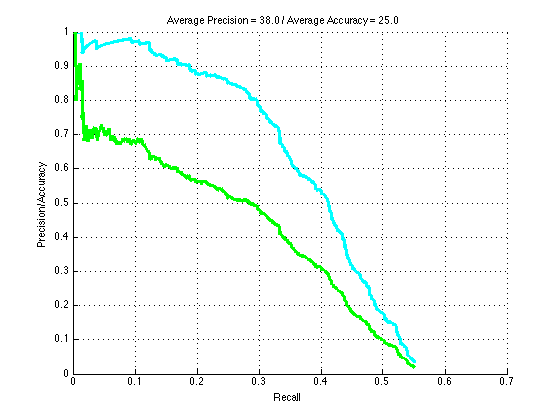
\includegraphics[width=\textwidth]{voc2012PRcnn4}
%               	\caption{3D-DPM CNN 4 views}
%        \end{subfigure}
%        \begin{subfigure}[b]{0.49\textwidth}
%                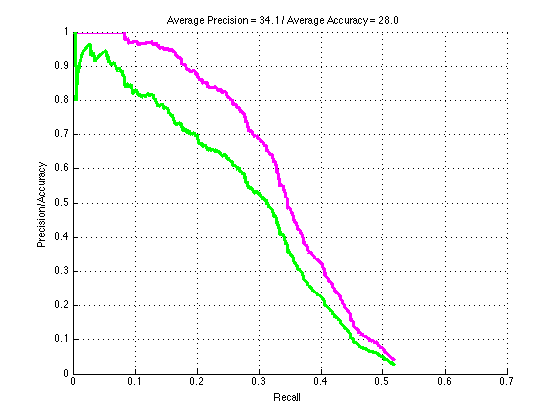
\includegraphics[width=\textwidth]{voc2012PRcnnPN4}
%                \caption{3D-DPM CNN-PN 4 views}
%        \end{subfigure}
%        \begin{subfigure}[b]{0.49\textwidth}
%                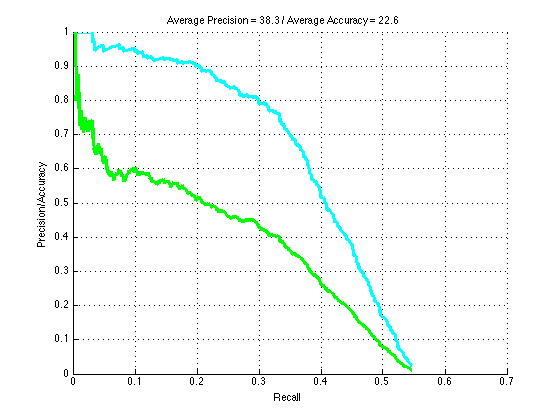
\includegraphics[width=\textwidth]{voc2012PRcnn8}
%               	\caption{3D-DPM CNN 8 views}
%        \end{subfigure}
%        \begin{subfigure}[b]{0.49\textwidth}
%                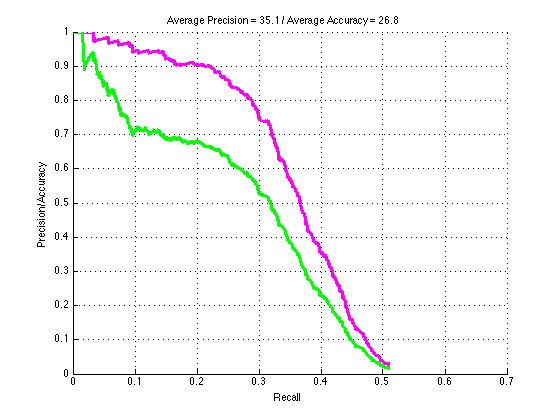
\includegraphics[width=\textwidth]{voc2012PRcnnPN8}
%                \caption{3D-DPM CNN-PN 8 views}
%        \end{subfigure}
%        \begin{subfigure}[b]{0.49\textwidth}
%                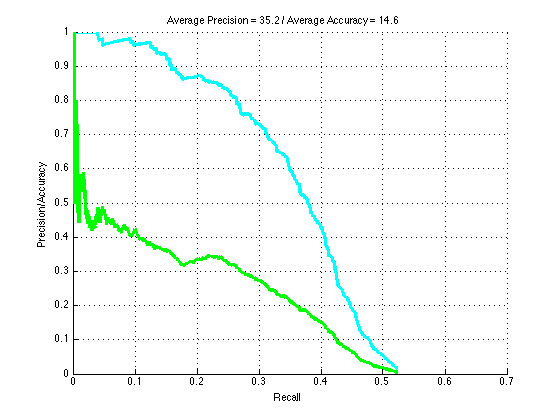
\includegraphics[width=\textwidth]{voc2012PRcnn16}
%               	\caption{3D-DPM CNN 16 views}
%        \end{subfigure}
%        \begin{subfigure}[b]{0.49\textwidth}
%                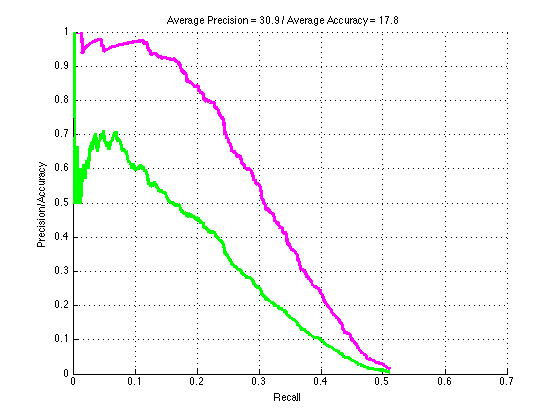
\includegraphics[width=\textwidth]{voc2012PRcnnPN16}
%                \caption{3D-DPM CNN-PN 16 views}
%        \end{subfigure}        
%\caption{Precision/Accuracy-Recall curves on VOC 2012 'val' of 3D-DPM CNN (left) and 3D-DPM CNN-PN (right). }
%\label{fig:voc2012cnn}
%\end{center}
%\end{figure}

In table \ref{tab:cnn2012} the performance of two CNN based models on VOC2012 'val' are shown in comparison to the HOG based 3D-DPM. The HOG based model doesn't make use of an extra octave, therefore making the feature pyramids of all the models comparable relative to their root size.  We can observe that the detection performance of 3D-DPM CNN is only slightly below the performance achieved  by 3D-DPM HOG. This is in accordance with recent work combining CNN features with DPMs \cite{girshick2014deformable} where the car category has shown to be one of only two categories where AP did not increase with CNN features while significantly improving the mean average precision (mAP) over all object categories (from 33.7 for HOG to 44.4 for CNN on VOC2007). While average precision is about on par with HOG based models, we can see that the viewpoint accuracy (VA) of 3D-DPM CNN is several points below the VA achieved by 3D-DPM HOG. This is due to a tendency observed in CNN based models to assign examples that are not viewpoint annotated to only a few model components. This results in detections that are concentrated on only those few components. As VA is arguably a better measure for the performance of a 3D-DPM as it directly measures the two main objectives of a 3D-DPM (object localisation and pose-estimation) we would like to increase the models VA performance. 3D-DPM CNN-PN uses positive examples with wrong viewpoint assignments as additional negative training examples. The intuition is that the model in this case learns to better distinguish between the different viewpoints of the object. As can be seen in table \ref{tab:cnn2012} the VA clearly improves with this training procedure while AP significantly decreases, and VA still not matching the performance of 3D-DPM HOG. %Figure \ref{fig:voc2012cnn} presents PR curves for the two CNN-based models on VOC 2012 'val'.


\begin{table}[]
	\begin{center}
		\begin{tabular}{|c|c|c|}
		\hline
		3D-DPM CNN & 3D-DPM CNN-PN & 3D-DPM HOG\\
		\hline\hline
		97.9/82.8 & 97.6/97.5 & 99.14/93.0\\
		\hline
		\end{tabular}
	\end{center}
\caption{Comparing the performance of CNN based models to a HOG based model using average precision and average viewpoint accuracy (AP/VA) on cars of the 3D object dataset \cite{4408987}.}\label{tab:cnn3ddataset}
\end{table}

%\begin{figure}
%\begin{center}
%	\begin{subfigure}[b]{0.49\textwidth}
%       		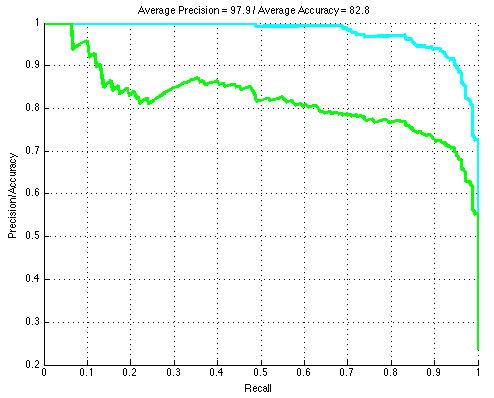
\includegraphics[width=\textwidth]{3ddataPRcnn}       
%                \caption{3D-DPM CNN}
%        \end{subfigure}
%        \begin{subfigure}[b]{0.49\textwidth}
%       		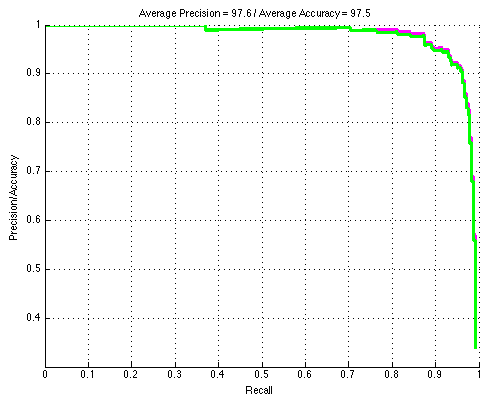
\includegraphics[width=\textwidth]{3ddataPRcnnPN}       
%                \caption{3D-DPM CNN-PN}
%        \end{subfigure}
%\caption{Precision/Recall and Viewpoint-Accuracy/Recall curves on cars of the 3D object dataset \cite{4408987}.}
%\label{fig:3ddataPRcnn}
%\end{center}
%\end{figure}

It is interesting to note however the results achieved on the 3D object dataset \cite{4408987} (listed in table \ref{tab:cnn3ddataset}). This dataset contains only cars in full sight, i.e. no truncated or occluded cars. Here 3D-DPM CNN-PN achieves the highest VA of all the models, also clearly outperforming the HOG based model. It is also noteworthy that AP and VA are nearly identical for 3D-DPM CNN-PN, therefore achieving the highest VA/AP ratio of all the models (see figure \ref{fig:PR3DDataset}).

Overall, the observation is that off-the-shelf CNN features do not lead to better results for 3D Deformable Parts Models on cars. It should be noted that the features used here were trained for image classification and that fine-tuning the parameters for object detection usually results in rather drastic performance improvements. 


